\documentclass[journal,12pt,twocolumn]{IEEEtran}
\usepackage{cite}
\usepackage{amsmath,amssymb,amsfonts,amsthm,mathtools}
\usepackage{algorithmic}
\usepackage{graphicx}
\parindent 0px
\bibliographystyle{IEEEtran}
\title{GATE 2023-EE Q49}
\author{EE23BTECH11052 - Abhilash Rapolu}
\begin{document}
\maketitle
\newpage
\textbf{Question 49}: The period of the discrete-time signal x[n] described by the equation below is N =\ (Round off to the nearest integer).
$$x[n] = 1 + 3\sin\left(\frac{15\pi}{8}n + \frac{3\pi}{4}\right) - 5\sin\left(\frac{\pi}{3}n - \frac{\pi}{4}\right)$$
\textbf{Solution:}
\begin{table}[htbp]
\centering
\begin{tabular}{|l|l|c|}
\hline
\textbf{Parameter} & \textbf{Description} & \textbf{Value} \\
\hline
$f_{1}$ & Sinusoid1 Frequency & 15/16 \\
\hline
$f_{2}$ & Sinusoid2 Frequency & 6 \\
\hline
\end{tabular}


\caption{Given parameters list}
\end{table}

The time period must be an integer for a discrete-time signal.

\begin{align}
T_1 &= \frac{1}{f_1} = \frac{16}{15} \\
T_2 &= \frac{1}{f_2} = 6 \\
N &= \text{LCM}(T_1, T_2) = 48
\end{align}

The Time Period of the signal is \(N = 48\).

Let's find the Z-transform of $x[n]$ by using the linearity property:

\begin{align}
X(z) &= Z(1) + Z\left(3\sin\left(\frac{15\pi}{8}n + \frac{3\pi}{4}\right)\right)\\
&\quad - Z\left(5\sin\left(\frac{\pi}{3}n - \frac{\pi}{4}\right)\right)\\
X(z) &= \sum_{n=-\infty}^{\infty} 1 \cdot z^{-n} \\
&\quad + \sum_{n=-\infty}^{\infty} (3\sin\left(\frac{15\pi}{8}n + \frac{3\pi}{4}\right) \cdot z^{-n} \\
&\quad + \sum_{n=-\infty}^{\infty} (5\sin\left(\frac{\pi}{3}n - \frac{\pi}{4}\right) \cdot z^{-n}\\
X(z) &= \frac{1}{1 - z^{-1}} + \frac{3\sin\left(\frac{3\pi}{4}\right)z}{z^2 - 2z\cos\left(\frac{15\pi}{8}\right) + 1} \\
&\quad - \frac{5\sin\left(-\frac{\pi}{4}\right)z}{z^2 - 2z\cos\left(\frac{\pi}{3}\right) + 1}\\
\Aboxed{X(z) &= \frac{1}{1 - 3\cos\left(\frac{15\pi}{8}\right)z^{-1} + z^{-2}} 
&\quad + \frac{5}{1 - 2\cos\left(\frac{\pi}{3}\right)z^{-1} + z^{-2}}} 
\end{align}
\begin{figure}[!ht] 
\centering
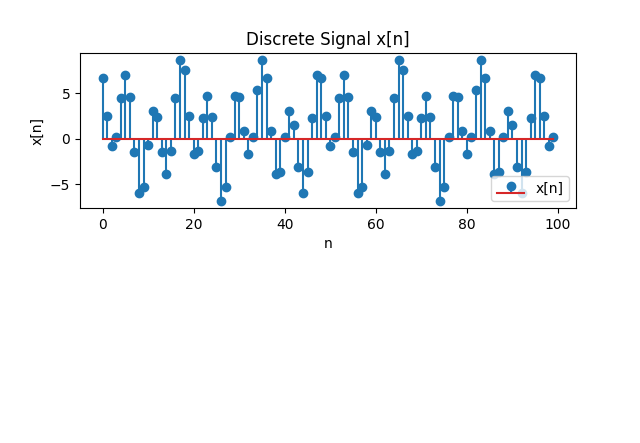
\includegraphics[width=2\columnwidth]{graph.png}
\label{fig:Graph1}
\end{figure}

\end{document}







